% Diagrama TikZ autocontido do Buffer Circular FIR (Etapa B - Pratica 3 PDS)
% Convencao do roteiro:
%   - Posicoes 1..N numeradas no sentido horario
%   - Escrita da nova amostra (idx_recente) avanca no sentido anti-horario
%   - Leitura das amostras (idx_leitura) percorre no sentido horario a partir de idx_recente
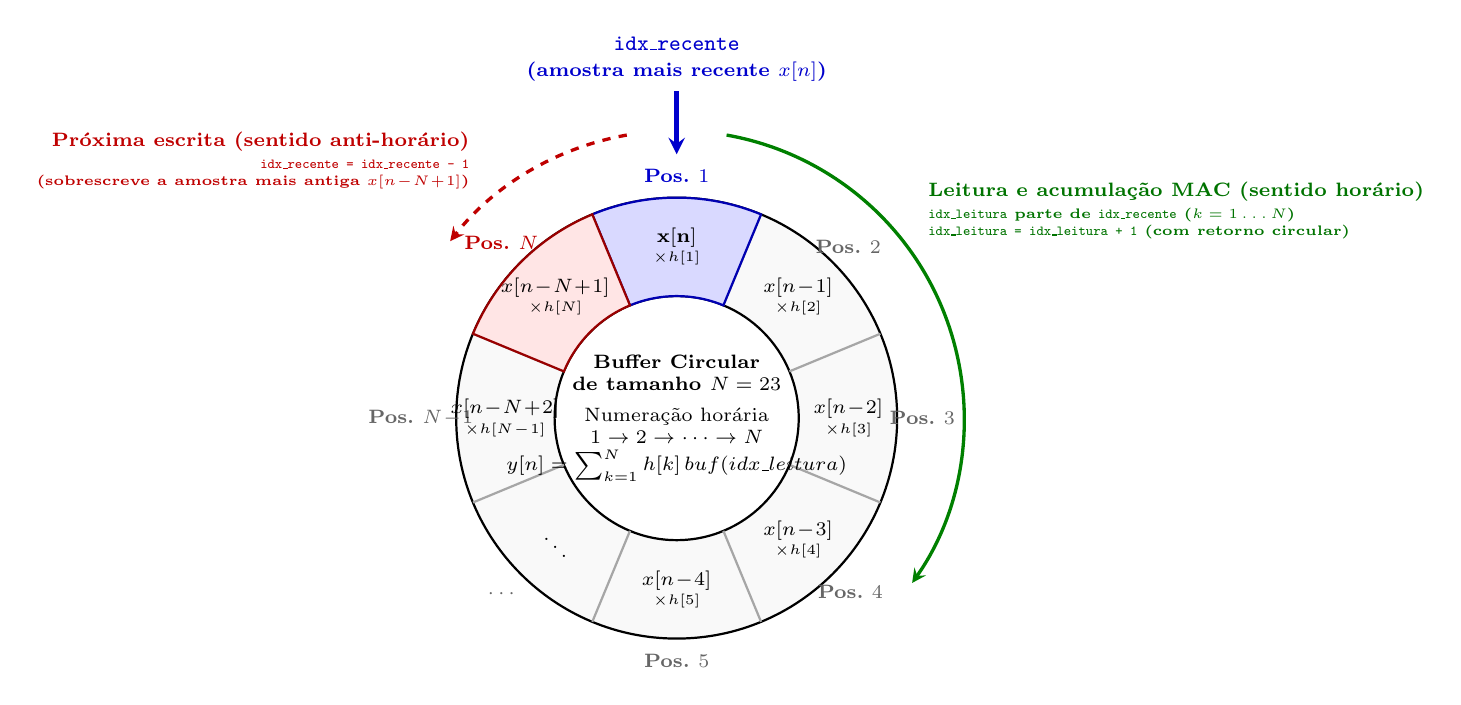
\begin{tikzpicture}[>=stealth, font=\small, scale=1.0]
    % Aneis de referencia do buffer circular
    \draw[thick, fill=gray!5] (0,0) circle (2.8cm);
    \draw[thick, fill=white]  (0,0) circle (1.55cm);

    % Divisoes radiais das 8 celulas ilustrativas (representando 1..N)
    \foreach \ang in {22.5, 67.5, 112.5, 157.5, 202.5, 247.5, 292.5, 337.5} {
        \draw[thick, gray!70] (\ang:1.55cm) -- (\ang:2.8cm);
    }

    % Destaque colorido para a celula atual de idx_recente (posicao 1 no topo, 90 graus)
    \fill[blue!15] (67.5:1.55cm) arc (67.5:112.5:1.55cm) -- (112.5:2.8cm) arc (112.5:67.5:2.8cm) -- cycle;
    \draw[thick, blue!70!black] (67.5:1.55cm) arc (67.5:112.5:1.55cm) -- (112.5:2.8cm) arc (112.5:67.5:2.8cm) -- cycle;

    % Destaque suave para a celula mais antiga (posicao N a esquerda do topo, 135 graus),
    % que sera sobrescrita no proximo passo anti-horario
    \fill[red!10] (112.5:1.55cm) arc (112.5:157.5:1.55cm) -- (157.5:2.8cm) arc (157.5:112.5:2.8cm) -- cycle;
    \draw[thick, red!60!black] (112.5:1.55cm) arc (112.5:157.5:1.55cm) -- (157.5:2.8cm) arc (157.5:112.5:2.8cm) -- cycle;

    % Numeracao das posicoes no sentido horario (1, 2, 3, 4, 5, ..., N-1, N)
    \node[font=\scriptsize\bfseries, blue!80!black] at (90:3.08cm)  {Pos.\ $1$};
    \node[font=\scriptsize\bfseries, gray!80!black] at (45:3.08cm)  {Pos.\ $2$};
    \node[font=\scriptsize\bfseries, gray!80!black] at (0:3.12cm)   {Pos.\ $3$};
    \node[font=\scriptsize\bfseries, gray!80!black] at (-45:3.12cm) {Pos.\ $4$};
    \node[font=\scriptsize\bfseries, gray!80!black] at (-90:3.08cm) {Pos.\ $5$};
    \node[font=\scriptsize\bfseries, gray!80!black] at (-135:3.15cm){$\cdots$};
    \node[font=\scriptsize\bfseries, gray!80!black] at (180:3.25cm) {Pos.\ $N\!-\!1$};
    \node[font=\scriptsize\bfseries, red!75!black]  at (135:3.15cm) {Pos.\ $N$};

    % Conteudo das amostras armazenadas e coeficientes associados na leitura horaria
    \node[align=center, font=\scriptsize] at (90:2.18cm)   {$\mathbf{x[n]}$\\[-1pt]{\tiny $\times h[1]$}};
    \node[align=center, font=\scriptsize] at (45:2.18cm)   {$x[n\!-\!1]$\\[-1pt]{\tiny $\times h[2]$}};
    \node[align=center, font=\scriptsize] at (0:2.18cm)    {$x[n\!-\!2]$\\[-1pt]{\tiny $\times h[3]$}};
    \node[align=center, font=\scriptsize] at (-45:2.18cm)  {$x[n\!-\!3]$\\[-1pt]{\tiny $\times h[4]$}};
    \node[align=center, font=\scriptsize] at (-90:2.18cm)  {$x[n\!-\!4]$\\[-1pt]{\tiny $\times h[5]$}};
    \node[align=center, font=\scriptsize] at (-135:2.18cm) {$\ddots$};
    \node[align=center, font=\scriptsize] at (180:2.18cm)  {$x[n\!-\!N\!+\!2]$\\[-1pt]{\tiny $\times h[N\!-\!1]$}};
    \node[align=center, font=\scriptsize] at (135:2.18cm)  {$x[n\!-\!N\!+\!1]$\\[-1pt]{\tiny $\times h[N]$}};

    % Ponteiro da amostra mais recente (idx_recente)
    \draw[->, ultra thick, blue!80!black] (90:4.15cm) -- (90:3.35cm);
    \node[above, align=center, font=\footnotesize\bfseries, blue!80!black] at (90:4.15cm)
        {\texttt{idx\_recente}\\{\scriptsize (amostra mais recente $x[n]$)}};

    % Seta anti-horaria de escrita (proxima posicao de escrita)
    \draw[->, very thick, red!75!black, dashed] (100:3.65cm) arc (100:142:3.65cm);
    \node[above left, align=right, font=\scriptsize\bfseries, red!75!black] at (132:3.75cm)
        {Próxima escrita (sentido anti-horário)\\{\tiny \texttt{idx\_recente = idx\_recente - 1}}\\[-2pt]{\tiny (sobrescreve a amostra mais antiga $x[n\!-\!N\!+\!1]$)}};

    % Seta horaria de leitura (idx_leitura) na parte interna/externa direita
    \draw[->, very thick, green!50!black] (80:3.65cm) arc (80:-35:3.65cm);
    \node[above right, align=left, font=\scriptsize\bfseries, green!45!black] at (35:3.75cm)
        {Leitura e acumulação MAC (sentido horário)\\{\tiny \texttt{idx\_leitura} parte de \texttt{idx\_recente} ($k = 1 \dots N$)}\\[-2pt]{\tiny \texttt{idx\_leitura = idx\_leitura + 1} (com retorno circular)}};

    % Texto central do anel
    \node[align=center, font=\scriptsize] at (0,0)
        {\textbf{Buffer Circular}\\\textbf{de tamanho $N = 23$}\\[3pt]Numeração horária\\$1 \rightarrow 2 \rightarrow \cdots \rightarrow N$\\[2pt]$y[n] = \sum_{k=1}^{N} h[k]\,\text{buf}(\text{idx\_leitura})$};
\end{tikzpicture}
